%++++++++++++++++++++++++++++++++++++++++
% Don't modify this section unless you know what you're doing!
\documentclass[letterpaper,10.8pt]{article}
\usepackage{natbib}
\usepackage{caption}
\usepackage{subcaption}
\bibliographystyle{unsrtnat}
\usepackage[super]{nth}
\usepackage{tabularx} % extra features for tabular environment
\usepackage{amsmath}  % improve math presentation
\usepackage{graphicx} % takes care of graphic including machinery


\usepackage[margin=0.7in,top=20mm,letterpaper]{geometry} % decreases margins

%\usepackage{cite} % takes care of citations
\usepackage[final]{hyperref} % adds hyper links inside the generated pdf file
\hypersetup{
	colorlinks=true,       % false: boxed links; true: colored links
	linkcolor=black,        % color of internal links
	citecolor=black,        % color of links to bibliography
	filecolor=magenta,     % color of file links
	urlcolor=black         
}
%+++++++++++++++++++++++++++++++++++++++
\begin{document}

\title{Natural Language Processing\\\textbf{Assignment 1}}

\author{D. Angelani\footnote{\href{mailto:davide.angelani@studio.unibo.it}{davide.angelani@studio.unibo.it}}, M. Ceresini\footnote{\href{mailto:marcello.ceresini@studio.unibo.it}{marcello.ceresini@studio.unibo.it}}, F. Cichetti\footnote{\href{mailto:federico.cichetti@studio.unibo.it}{federico.cichetti@studio.unibo.it}}, G. Ruberto\footnote{\href{mailto:giuseppe.ruberto2@studio.unibo.it}{giuseppe.ruberto2@studio.unibo.it}}}

\date{\today}

\maketitle

\begin{abstract}
In this relation we explain how we addressed the task of Part of Speech (POS) tagging i.e. the process of assigning to each word in a sentence its correct syntactic category. After reporting our pre-processing pipeline, we showcase our experiment with the proposed networks. From our experiments, we report that using GRUs instead of LSTMs and deepening the classifier head of the network were the most successful modifications to the baseline architecture. We reached a $0.740$ F1-Macro score on the validation set with our best model, and with further analysis we show how the most common errors of the network often reflect frequent human mistakes.
\end{abstract}

\tableofcontents

\newpage

\section{Description of the Task}

A part-of-speech (POS) is a category of words with similar grammatical properties. POS tagging is the task where, given a sentence from a corpus of documents, we need to predict the POS tag of each word. It is a useful task when dealing with disambiguation of words within a sentence\footnote{e.g. Is \emph{book} a noun or a verb? Of course, it depends on the context.}. Naturally, the task can be cast as a \emph{classification} problem: given a sequence of tokens $X = [x_1, \dots, x_n]$ produce a sequence of tags $Y = [y_1, \dots, y_n]$ such that: \begin{gather*} y_i = argmax_{c \in C}(f(x_i)) = argmax_{c \in C}([y_i^{c_1}, \dots, y_i^{c_n}]), i=1 \dots n\end{gather*}

\section{Dataset and Preprocessing}
\subsection{Dataset Analysis}
The dataset is composed of several files, each containing a paragraph of tokenized text composed by one or more sentences. We decided to deal with sentences rather than entire paragraphs, so we built some functions to split the text in the files whenever a dot tag is found (usually corresponding to \texttt{'.', '!' or '?'}).

Each word in the dataset is tagged with its own ground truth POS tag. The set of tags used in our dataset is the one popularized by the \href{https://www.ling.upenn.edu/courses/Fall_2003/ling001/penn_treebank_pos.html}{\emph{Penn Treebank Project}}, plus some punctuation tags (\texttt{["\#", "\$", "''", ",", ".", ":", "``", "-LRB-", "-RRB-"]}). We consider the \textt{"SYM"} tag also a punctuation tag, so in total there are $11,715$ punctuation tags in the dataset over $94,081$ total tags ($12.45\%$). The distribution of tags is slightly skewed towards some of the classes (Figure \ref{fig:label_distr}): some of the less represented ones could represent an obstacle for our models.

The dataset splits are already provided: there are $1959$ sentences in the training set, $1277$ in validation and $638$ in test (Figure \ref{fig:sentence_distr}). Sentences seem to have approximately the same length distribution between the three splits, with an average of $\sim 24$ words per sentence, but there are some clear outliers in the training set (Figure \ref{fig:sentence_len}). 

\subsection{Embeddings and OOV terms}
As for pre-processing, since the goal of the task is to provide a one-to-one mapping between tokens and tags, it was important not to remove any of the tokens from the dataset splits. Thus, we only applied a lowercase transformation to the tokens.

We matched our tokens to GloVe's pre-trained dense embeddings (with a dimensionality of $100$) and then created sensible encodings for OOV (Out-Of-Vocabulary words, that were not present in GloVe's vocabulary). We processed the OOV terms of each split independently by progressively constructing our vocabulary: from GloVe's vocabulary we firstly added OOVs from the train set; then we added to this larger vocabulary the OOVs from the validation set and finally we repeated the precedure with the test set.

OOV embeddings are random vectors with the same dimensionality as the original encodings, sampled from a uniform distribution using the mean and standard deviation computed from the set of GloVe's embeddings, so that the distributions of real and OOV embeddings are similar.

The sets of OOV terms for all splits seem to follow the same pattern: they mostly contain hyphenated compound words, numbers, foreign or other uncommon words. The number of OOV terms is always less than $5\%$ in all splits ($4.85\%$ in the training split, $3.49\%$ in the validation split and $3.76\%$ in the test split), so we believe they did not impact our results too much.

\subsection{Padding}
In order to be able to provide batches of sentences to the networks, we chose to apply padding to force all sequences to have the same length. We shifted the embedding matrix to the right by one position, so that the padding token could have index 0 in the vocabulary. This is useful because in Keras there are options for the embedding layer to automatically produce masks so that the recurrent layers will completely ignore padding tokens, speeding up the training procedure.

Traditional padding brings all tensors to the same shape of the longest, but with our analysis we discovered that the longest sequence of tokens in the training set contains $250$ elements\footnote{This is hidden in Figure \ref{fig:sentence_len} because clear outliers were cut for more visual clarity.}. Clearly, forcing all sequences to have over $10$ times more than their average number of elements is a waste of memory.

We decided to fix the maximum length at $80$, which is the maximum length between validation and test splits. By doing so, only $5$ sentences of the training set over $1959$ ($0.2552\%$) need to be \emph{truncated} (only the first $80$ tokens are kept), while memory consumption is reduced by $\frac{1}{3}$.

\section{Models Description}

The networks receive a (padded) sequence of \emph{indices} that refer to the position of each token in the vocabulary we have built, and produce probability distributions over the $46$ tags for each of the $80$ tokens of the sentence. Thus, both input and output are tensors of shape $[batch\_size, 80, 46]$\footnote{In our experiments, $batch\_size$ is always $128$.}. 

\iffalse
We use \href{https://www.tensorflow.org/api_docs/python/tf/data/Dataset}{TensorFlow's \emph{Dataset} class} to automatically deliver batched inputs and their ground truth labels to the models. Additionally, 
\fi

All models are implemented using \href{https://keras.io/guides/functional_api/}{Keras's Functional API}. The embedding layer's weights are initialized with our embedding matrix and are non-trainable. The Bidirectional wrapper for the recurrent layer(s) is programmed to concatenate the output of the two recurrent processes, so whatever number of units for the recurrent layer is set, the real output is always doubled\footnote{For example, the baseline uses a $128$-units Bidirectional LSTM layer, so the output has shape $[batch\_size, 80, 256]$.}. The classifier is implemented with a \href{https://keras.io/api/layers/recurrent_layers/time_distributed/}{\emph{time-distributed}} fully connected layer, so that each sentence in the batch undergoes the same processing independently from others. Variations of the baseline include: using a layer of GRU cells rather than LSTM, adding a FC layer to the classifier or adding a Bi-LSTM layer in the recurrent part. We use the Adam optimizer for all of our experiments and sparse categorical crossentropy loss, since the ground truth tags are provided as simple indices rather than one-hot encoded vectors for efficiency. 

We also employ \emph{early stopping} monitoring the validation accuracy with a patience of 10 epochs, but apply no further regularization because no extreme signs of overfitting were noticed. The training was set up to have a maximum of $70$ epochs, but due to early stopping all training experiments usually halted after $25$-$40$ epochs 

\section{Results}

As instructed, we use the $\operatorname{F1-Macro}$ score\footnote{Average of F1-Scores computed on each class:$ \frac{1}{N}\sum^N_{i=0}\operatorname{F1-Score}_i$} to evaluate models without considering the punctuation classes. We noticed that since the embedding layer is \emph{masking} the padding tokens, the neural network is completely ignoring them and always predicts the "dot" class (.) for a PAD, probably because it has learnt that a sentence always ends with a dot. Anyway, we also discard PAD tokens while estimating the $F1$ score.

We showcase our results on the validation and test set (only for the two best scoring models on the validation split) with this table:

\begin{center}
\begin{tabular}{c | c  c  c  c }
    $F1-Macro$ & baseline & gru & deeper\_dense & deeper\_lstm  \\
    \hline
    validation & 0.7345 & 0.7669 & 0.7552 & 0.7209 \\
    test       &    -   & 0.7333 & \textbf{0.7393} & - \\
\end{tabular}
\end{center}


It's important to note that during our training experiments, the classification results varied due to randomness in the process, but overall were approximately comparable to the ones presented here. 

We selected the GRU model and the model using two fully-connected layers as our best-scoring models.

\section{Error analysis}

We analyzed the errors of the best models on the test set by computing the confusion matrices (Figure \ref{fig:confusion_matrices}). 6 tags in particular are responsible for about $70\%$ of the mistakes of the models: JJ (adjectives), NN (singular nouns), NNP (proper nouns), NNS (plural nouns), RB (adverbs) and VBN (past principle verbs). Namely, singular, plural, proper nouns and adjectives are sometimes confused with each other and some adverbs are predicted as adjectives (and vice-versa): most of these are common mistakes even for humans! By printing some of the specific sentences where commons errors are made, we looked for patterns in the mistakes.

Let's take for example these sentences:
\iffalse
\begin{itemize}
   \item sales totaled 1.916 trillion yen, climbing $17\%$ from $1.637$ trillion yen in the year-earlier period .
   \item the recent rally in precious metals was a result of uncertainty and volatility in equities, he said 
   \item but it is particularly difficult this autumn because of low water levels on the mississippi river, on which flows much of the u.s. corn that is shipped overseas.
   \item but the two legal experts, responding to an inquiry by sen. edward kennedy (d. , mass.), wrote in a joint letter that the president lacks the constitutional authority to exercise a line-item veto.
\end{itemize}
\fi

\begin{center}
\scalebox{0.7}{%
\begin{tabular}{c | c  c  c  c  c  c  c  c  c  c  c  c  c  c  c  c  c  c }
    word & sales & totaled & 1.916 & trillion & yen & , & climbing & 17 & \% & from & 1.637 & trillion & yen & in & the & year-earlier & period & .  \\
    \hline
    tag & NNS & VBD & CD & CD & NN & , & VBG & CD & NN & IN & CD & CD & NN & IN & DT & JJ & NN & . \\
    prediction & NNS & VBD & CD & CD & \textcolor{red}{NNS} & , & VBG & CD & NN & IN & CD & CD & \textcolor{red}{NNS} & IN & DT & JJ & NN & . \\
\end{tabular}}
\end{center}

\begin{center}
\scalebox{0.7}{%
\begin{tabular}{c | c  c  c  c  c  c  c  c  c  c  c  c  c }
    word & it & is & n't & clear & how & much & a & restructuring & would & help & columbia & stockholders & .\\
    \hline
    tag & PRP & VBZ & RB & JJ & WRB & JJ & DT & NN & MD & VB & NNP & NNS & .\\
    prediction & PRP & VBZ & RB & JJ & WRB & \textcolor{red}{RB} & DT & NN & MD & VB & NNP & NNS & .\\
\end{tabular}}
\end{center}



The model confuses words regarding money for plural: it makes sense because they are predeced by plural numbers. Also, a common pattern seems to be that the model may think that abstract concepts (volatility, demand, \dots) are plural. \textit{"Moreover", "much", "enough", ...} are all sources of problems because they can be both adjectives and adverbs depending on the context. From the last example we can see that adjectives that are pretty specific and complex may lead the model to believe that they are representative enough to be nouns. Anyway, the network shows many signs of understanding context correctly and more often than not predicts the correct tags.

\newpage

\section{Appendix: Figures}

\begin{figure}[ht]
    \centering
    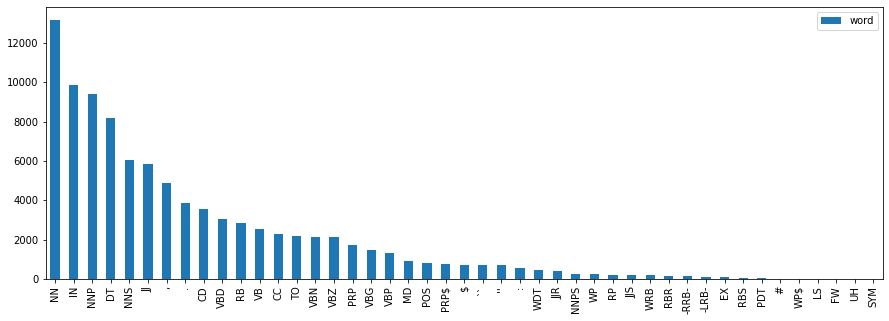
\includegraphics[width=\textwidth]{imgs/label_distr.png}
    \caption{Distribution of tags on the whole dataset}
    \label{fig:label_distr}
    \hfill
\end{figure}

\begin{figure}[ht]
    \begin{subfigure}[t]{0.43\textwidth}
        \centering
        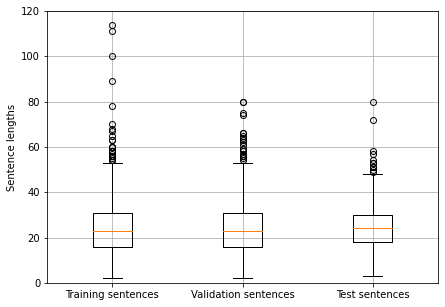
\includegraphics[width=\textwidth]{imgs/len_distr.png}
        \caption{Distribution of sentences lengths across the 3 splits.}
        \label{fig:sentence_len}
    \end{subfigure}
    \hfill
    \begin{subfigure}[t]{0.54\textwidth}
        \centering
        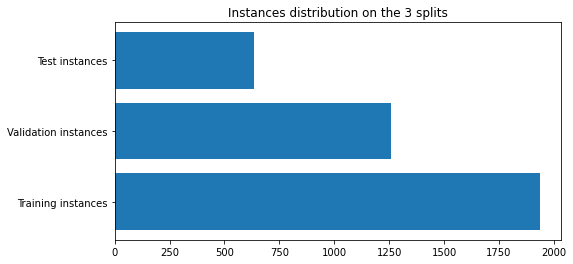
\includegraphics[width=\textwidth]{imgs/split_distrib.png}
        \caption{Distribution of sentences in the 3 splits.}
        \label{fig:sentence_distr}
    \end{subfigure}
    \caption{Composition of the train/val/test splits in the dataset.}
\end{figure}

\begin{figure}
    \begin{subfigure}[t]{0.485\textwidth}
        \centering
        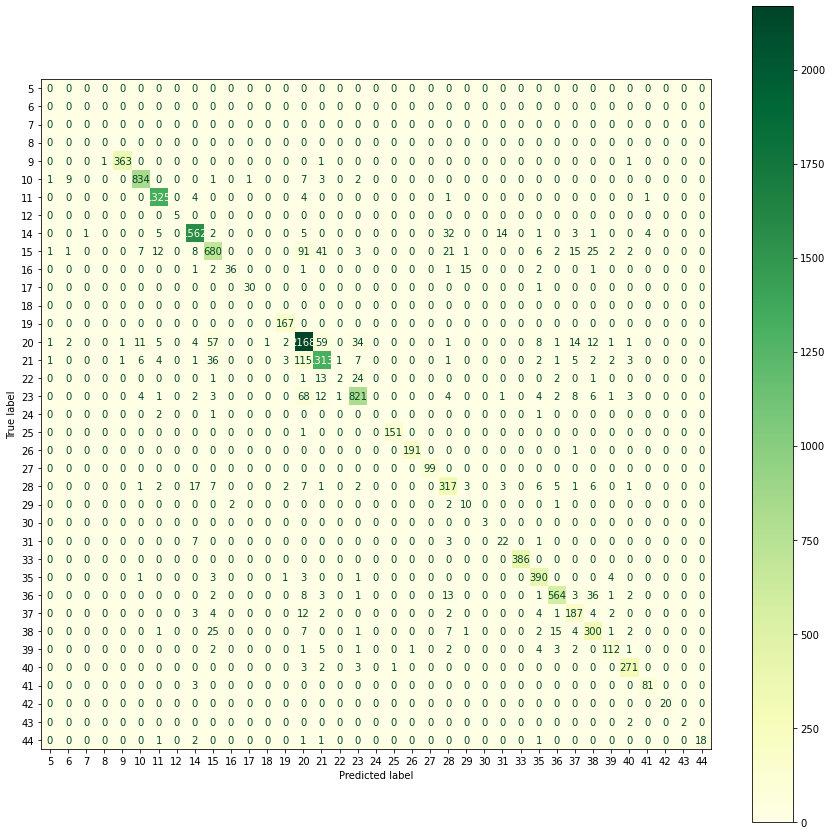
\includegraphics[width=\textwidth]{imgs/deeper_classifier.png}
        \caption{Performance of the deeper-classifier model on the test set.}
        \label{fig:performance_deeper}
    \end{subfigure}
    \hfill
    \begin{subfigure}[t]{0.485\textwidth}
        \centering
        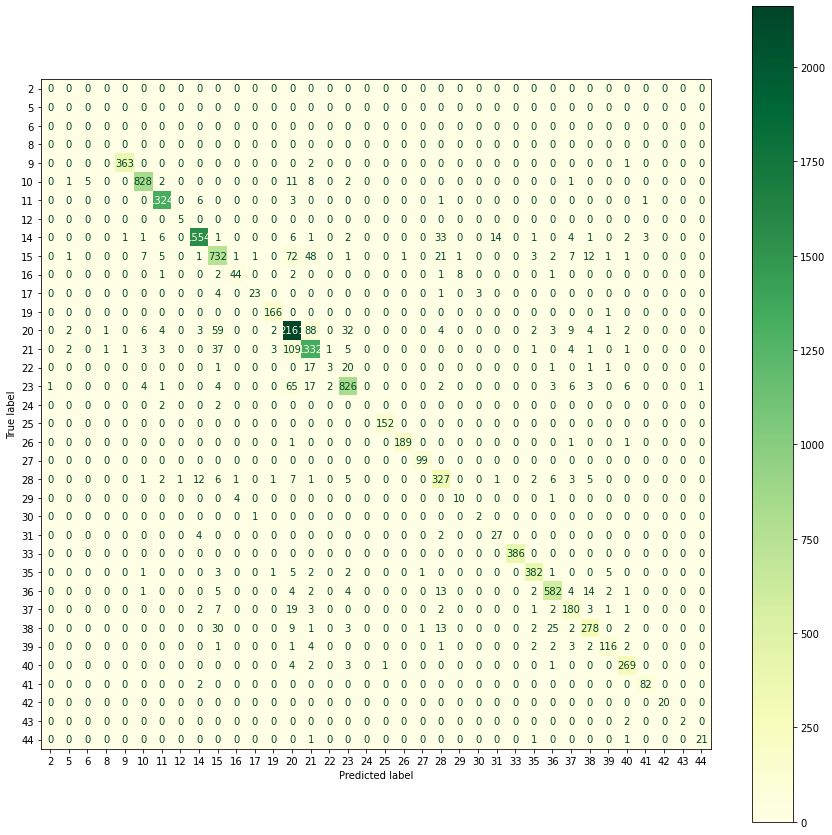
\includegraphics[width=\textwidth]{imgs/gru.png}
        \caption{Performance of the GRU model on the test set.}
        \label{fig:performance_gru}
    \end{subfigure}
    \caption{Confusion matrices of our best models over the test split.}
    \label{fig:confusion_matrices}
\end{figure}
\end{document}

